\chapter{State of the Art}
\label{chap:state_of_art}
\section{Cooperative Cable-Driven Aerial Systems}

Several robotic architectures can be considered for the manipulation of a payload using multiple aerial vehicles. Among them, Cable-Driven Parallel Robots (CDPRs), Aerial Cable-Towed Systems (ACTSs), and Flying Parallel Robots (FPRs) are particularly relevant to the problem considered in this thesis. These architectures differ mainly in how the payload is connected to the actuators and consequently in their workspace, force-generation capabilities, and mechanical complexity.

\subsection{Aerial Cable-Towed Systems}

An Aerial Cable Towed Robot (ACTR) is a robotic system where the load is connected to multi-rotor UAVs through cables \cite{xiong_optimal_2022}. Other cables may be actuated also by non-aerial devices, such as actuators fixed to the ground or UGVs. In these systems, the payload motion is achieved by coordinating the cable tensions generated by the different actuators. 

While standard ACTRs are limited in the directions and magnitudes of forces they can generate, the combination of mobile UAVs and fixed ground anchors enables the system to adapt its available wrench set to task requirements. This allows the platform to exert higher and more controllable interaction forces compared to configurations without a ground-based tension reference \cite{jamshidifar_static_2020}.

\begin{figure}[ht]
    \centering
    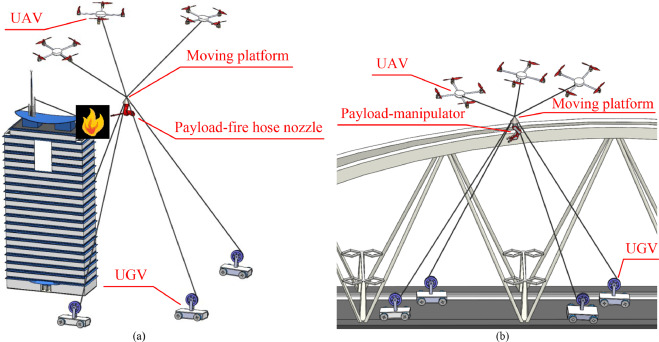
\includegraphics[width=0.75\linewidth]{Images/ACTR-graphicalRepresentation.jpg}
    \caption{ACTRs with land-fixed winches for firefighting applications (a) and repair of a large bridge (b) \cite{xiong_optimal_2022}}
    \label{fig:ACTRgraphicalRepresentation}
\end{figure}

\subsection{Cable-Driven Parallel Robots}
\label{sec:Cable-DrivenParallelRobots}
In conventional CDPRs, the end-effector is manipulated through flexible cables connected to fixed anchor points on the ground, and its motion is controlled by adjusting the cable lengths. Although CDPRs do not employ aerial robots, their analysis can be beneficial for making progress on ACTSs. As proposed by \cite{erskine_control_2019}, ACTSs can be interpreted as reconfigurable CDPRs (RCDPRs), where fixed anchor points are replaced by mobile aerial platforms. For this reason, existing results on CDPR kinematics, dynamics, and control should not be ruled out a priori. 
A fundamental difference between CDPRs and ACTSs lies in the available tension space. In classical CDPR the tension's limits are fixed and do not depend on the robot's pose: the minimum tension is usually a small positive value to avoid slack, while the maximum tension is set by the motor torque. On the other hand, UAVs in ACTSs must always generate enough thrust to keep itself in the air and maintain its attitude, reducing the tension margin available for payload manipulation \cite{erskine_wrench_2019}. Therefore, CDPR findings can still be used for ACTSs, but they need to be adapted by introducing additional constraints due to the quadrotor actuation limits \cite{erskine_control_2019, masone_cooperative_2016}. 

\begin{figure}[h]
    \centering
    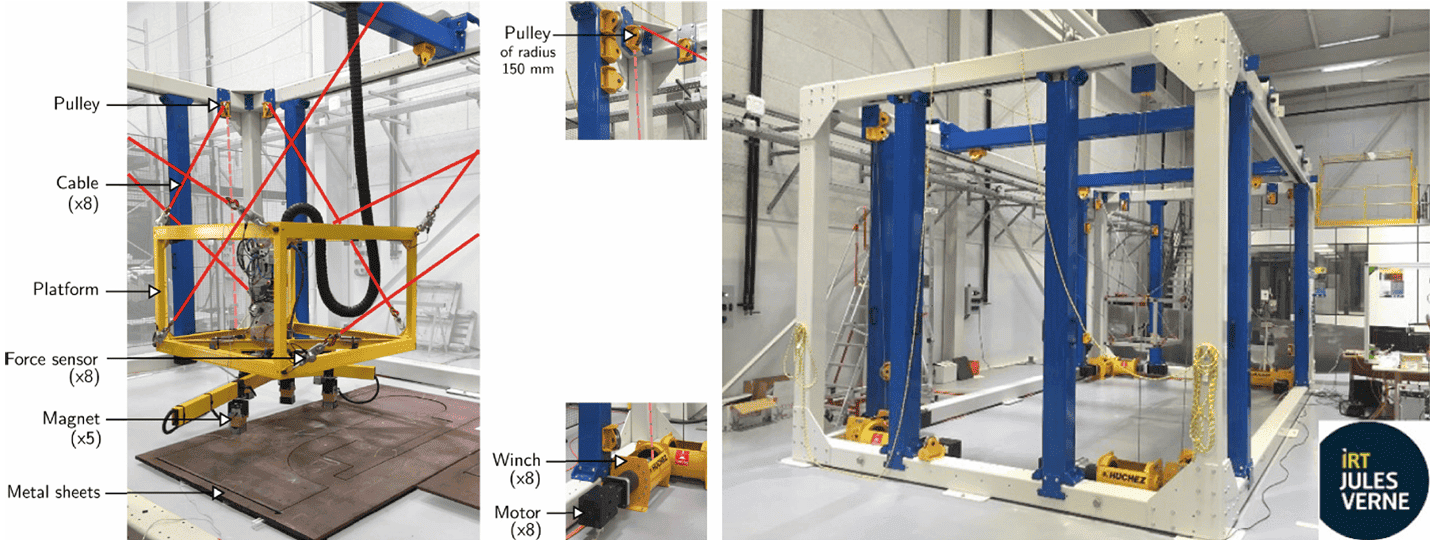
\includegraphics[width=\linewidth]{Images/CDPRschematics.png}
    \caption{CDPR located at IRT Jules Verne \cite{pott2013cable, Picard2018}}
    \label{fig:CDPRschematics}
\end{figure}

\subsection{Flying Parallel Robots}
Flying Parallel Robots (FPRs) changes from the previous two designs in that they connect the UAVs to the manipulated platform by rigid connections rather than cables, allowing both pushing and pull forces to be transmitted. The rigid legs also incorporate passive joints, providing additional passive degrees of freedom within the kinematic chains. These joints can reorient without actuation, preventing the platform from becoming over-constrained while maintaining the ability to transmit compressive loads \cite{liu_wrench_2022}. This makes FPRs particularly well suited for tasks involving sustained physical interaction with the environment. However, the rigid links significantly increase the system's weight and mechanical complexity compared with cable-based architectures \cite{six_dynamic_2021}.

ACTSs achieve a similar interaction objective relying on coordinated control of multiple cable tensions. When ground anchors or UGVs are incorporated, the system can generate the reaction forces required for façade interaction while preserving the lightweight and mechanically simple nature of cable-driven robots.
\begin{figure}[h]
    \centering
    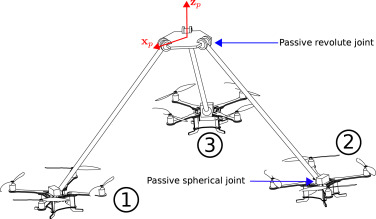
\includegraphics[width=0.55\linewidth]{Images/FPR-schematics.jpg}
    \caption{Kinematic scheme of the 3-DSR flying parallel robot \cite{six_dynamic_2021}}
    \label{fig:FPRschematics}
\end{figure}


\section{Interaction with the Environment}
Physical interaction is particularly challenging for aerial robotic systems because, unlike ground-based manipulators with a fixed base, aerial vehicles must simultaneously generate the forces required to remain airborne and those required to interact with the environment. Aerodynamic disturbances and modelling uncertainties further complicate the control problem \cite{liu_wrench_2022}. In a cable-suspended system, these effects are coupled: a change in the position of one UAV or of the payload modifies the cable directions and consequently the forces experienced by the other agents \cite{sun_agile_2025}.

These challenges become particularly important when the payload operates close to a vertical surface. Accuracy is a critical requirement in such applications, and interaction with the environment introduces additional force constraints that are not present during free-space motion \cite{jamshidifar_static_2020}. Near-façade operation can also be affected by aerodynamic phenomena. Ground and ceiling effects modify the UAV dynamics, while the propeller wash generated by one UAV can disturb other vehicles operating in proximity \cite{six_dynamic_2021, sun_agile_2025}. Furthermore, uncertainties in payload mass and inertia can affect the required thrust and lead to tracking errors or actuator saturation \cite{erskine_control_2019, sun_agile_2025}.

Several forms of interaction have been considered for ACT systems, including unexpected collisions, planned contact, and active interaction with an external agent \cite{sanalitro_indirect_2022}. For the FaçadeShieldBot application, the relevant case is planned physical interaction with a vertical surface.




\section{Control of Cable-Suspended UAV Systems}

\subsection{Control Architecture}

Control architectures for cooperative aerial transportation can broadly be classified as centralized, distributed, or decentralized. In a centralized architecture, information about the UAVs, payload, and system configuration is available to a common controller. This allows the controller to coordinate the agents and explicitly account for the coupling between their motions.

A common approach is to model the ACTS as a continuously reconfigurable cable-driven parallel robot. In this framework, the controller can coordinate the payload motion, cable tensions, and UAV motion within a single control architecture \cite{masone_cooperative_2016, erskine_control_2019}.

In \cite{masone_cooperative_2016}, the design of a centralized trajectory tracking controller is proposed that explicitly accounts for both the kinematics and dynamics of the system. The control architecture is structured into three main layers:
\begin{itemize}
    \item A task-space control loop that computes the desired wrench acting on the payload;
    \item A tension distribution algorithm that determines a feasible set of cable tensions realizing that desired wrench; and
    \item A joint-space control loop that converts the required cable forces into thrust and attitude commands for each quadrotor.
\end{itemize}

In contrast, distributed control architectures do not rely on a single controller. Instead, each UAV computes its control action using locally available information while exchanging information with neighbouring agents to achieve a common objective. Consensus algorithms are commonly employed to estimate global quantities, such as the payload state or formation geometry, without requiring complete knowledge of the system \cite{erskine_dynamic_2021}. Decentralized control assumes that each UAV relies solely on its own local measurements, without explicit information exchange with the other agents. In this case, preserving the formation geometry becomes critical.

The system considered here is assumed to operate under centralized control, for which the states and configuration of the relevant agents are available to a common controller.


\subsection{Cable Tension and Force Control}

Cable tension management is fundamental to the control of cable-driven systems because cables can only transmit tensile forces. The controller must therefore ensure that the tensions remain positive to prevent cable slackness and maintain the desired mechanical configuration.

In redundant cable-driven systems, several sets of cable tensions can generate the same net wrench on the payload. This redundancy can be exploited to satisfy additional constraints while maintaining the desired payload wrench. In particular, internal forces corresponding to the null space of the wrench mapping can be used to modify the tension distribution without changing the resulting payload wrench \cite{masone_cooperative_2016, jamshidifar_static_2020}.

For ACTSs, tension feasibility is further constrained by the UAVs' actuation limits. Each UAV must allocate part of its available thrust to compensate for its own weight and maintain its attitude, leaving only a limited portion of its actuation capability for payload manipulation \cite{erskine_wrench_2019}. A valid control solution must therefore consider both the desired payload wrench and the available actuation capabilities.

More recent approaches incorporate cable tension constraints directly into trajectory optimization, allowing future trajectories to be evaluated according to their feasibility with respect to cable tension and actuator limits \cite{sun_agile_2025}. Such approaches demonstrate the importance of considering cable forces explicitly when planning or controlling cooperative aerial systems.

\section{Positioning of this work in the current state of the art}
% How can an ACTS architecture be designed before building the robot? How should UAV and ground cable attachment points be selected?

Existing research on ACTS has focused primarily on modeling, trajectory generation, and controller design. In contrast, little attention has been paid to the systematic design of the architecture itself. In particular, selecting the number and placement of cable attachment points and choosing appropriate cable routes. These decisions directly influence the set of achievable torques, controllability, workspace, robustness, and the performance of any controller.

% How can feasible cable routings be automatically identified among many possibilities?

This thesis addresses these challenges by proposing a methodology for the design and evaluation of aerial cable-towing systems (ACTS) that combine UAVs and ground anchors. First, a general kinematostatic model is developed to describe ACTS architectures. Based on this model, a comprehensive preselection study is introduced to identify feasible cable configurations that satisfy the constraints of wrench closure, wrench feasibility, and interference constraints. The candidate architectures are then evaluated using both geometric performance indices and closed-loop dynamic simulations employing the proposed control framework.

% Which performance metrics are truly predictive of practical manipulation performance? How can theoretical architecture evaluation be connected with dynamic closed-loop simulations?

Particular attention is given to the positioning of UAV attachment points and the arrangement of ground anchors, providing a quantitative comparison of various possible configurations. Thanks to the proposed methodology, it will be possible to design, evaluate, and select ACTS architectures, bridging the gap between the theoretical analysis of cable-controlled robots and the practical implementation of collaborative aerial manipulation systems.